\begin{figure}[H]
    \centering
    \begin{adjustbox}{max width=\textwidth}
        \centering
        % Scale factor 0.024395857307249712
\definecolor{color0}{RGB}{222,239,234}
\definecolor{color1}{RGB}{192,192,192}
\definecolor{color2}{RGB}{153,153,255}
\definecolor{color3}{RGB}{255,153,153}
\definecolor{color4}{RGB}{255,255,255}
\definecolor{color5}{RGB}{255,255,153}
\definecolor{color6}{RGB}{153,255,153}
\definecolor{color7}{RGB}{0,150,60}
\definecolor{color8}{RGB}{170,30,30}
\definecolor{color9}{RGB}{255,0,0}
\definecolor{color10}{RGB}{100,100,255}
\definecolor{color11}{RGB}{0,0,0}
\definecolor{color12}{RGB}{128,0,128}
% Bounding Box: 968.0, 869.0
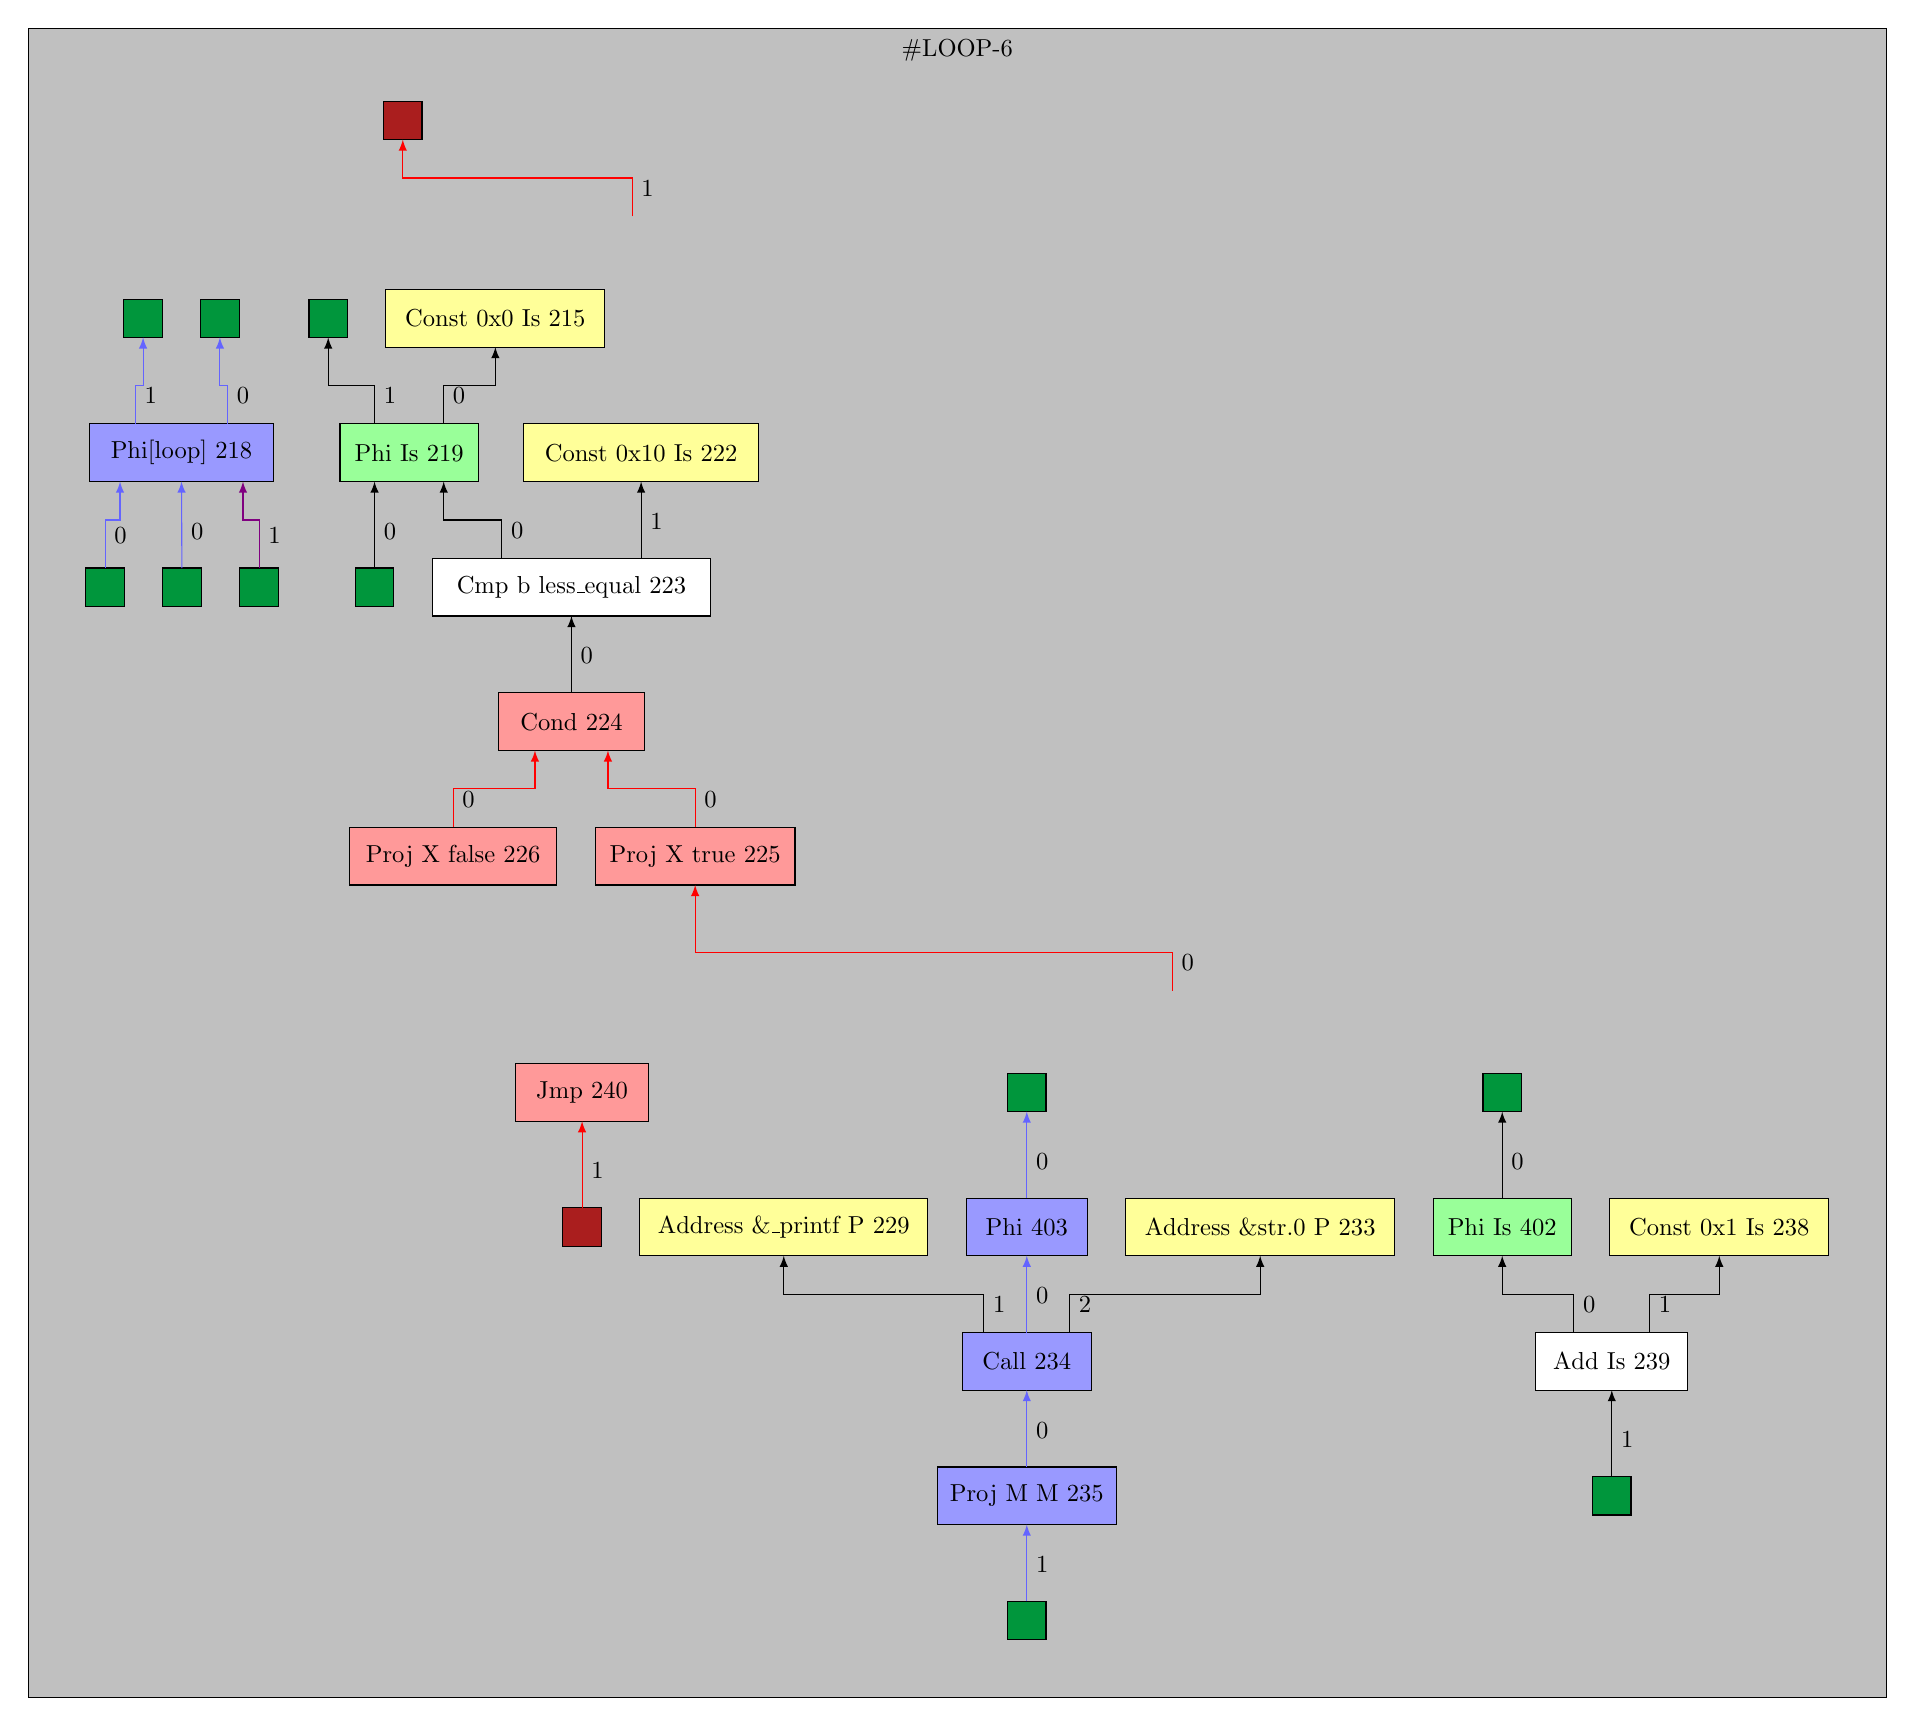
\begin{tikzpicture}
	\node[fill=color0, draw, minimum width=17.40644418872267cm, minimum height=8.611737629459148cm] (n1) at (14.895584286649068cm ,-2.427387802071346cm) {};
	% 1 node layouts
	\node[scale=0.8871220838999895, transform shape] at (14.895584286649068cm ,1.599834579976985cm) {Block  227};
	\node[fill=color0, draw, minimum width=9.73825221688215cm, minimum height=8.855696202531645cm] (n2) at (5.601001827658567cm ,7.282163406214039cm) {};
	% 1 node layouts
	\node[scale=0.8871220838999895, transform shape] at (5.601001827658567cm ,11.431365074798618cm) {Block  217};
	\node[fill=color1, draw, minimum width=23.5988063810104cm, minimum height=21.2cm] (n3) at (12.165341050113947cm ,3.5008055235903335cm) {};
	% 1 node layouts
	\node[scale=0.8871220838999895, transform shape] at (12.165341050113947cm ,13.822159090909091cm) {\#LOOP-6};
	\node[fill=color2, draw, minimum width=2.342002301495972cm, minimum height=0.7318757192174914cm] (n4) at (2.312583767684289cm ,8.709321058688147cm) {};
	% 1 node layouts
	\node[scale=0.8871220838999895, transform shape] at (2.312583767684289cm ,8.709321058688147cm) {Phi[loop]  218};
	\node[fill=color3, draw, minimum width=2.634752589182969cm, minimum height=0.7318757192174914cm] (n5) at (5.761727475800447cm ,3.5861910241657076cm) {};
	% 1 node layouts
	\node[scale=0.8871220838999895, transform shape] at (5.761727475800447cm ,3.5861910241657076cm) {Proj X false 226};
	\node[fill=color3, draw, minimum width=2.53716915995397cm, minimum height=0.7318757192174914cm] (n6) at (8.83560549651391cm ,3.5861910241657076cm) {};
	% 1 node layouts
	\node[scale=0.8871220838999895, transform shape] at (8.83560549651391cm ,3.5861910241657076cm) {Proj X true 225};
	\node[fill=color3, draw, minimum width=1.854085155350978cm, minimum height=0.7318757192174914cm] (n7) at (7.264942801055981cm ,5.293901035673187cm) {};
	% 1 node layouts
	\node[scale=0.8871220838999895, transform shape] at (7.264942801055981cm ,5.293901035673187cm) {Cond  224};
	\node[fill=color4, draw, minimum width=3.5373993095512084cm, minimum height=0.7318757192174914cm] (n8) at (7.264942801055981cm ,7.001611047180667cm) {};
	% 1 node layouts
	\node[scale=0.8871220838999895, transform shape] at (7.264942801055981cm ,7.001611047180667cm) {Cmp b less\_equal 223};
	\node[fill=color5, draw, minimum width=2.9762945914844647cm, minimum height=0.7318757192174914cm] (n9) at (8.149292628443783cm ,8.709321058688147cm) {};
	% 1 node layouts
	\node[scale=0.8871220838999895, transform shape] at (8.149292628443783cm ,8.709321058688147cm) {Const 0x10 Is 222};
	\node[fill=color6, draw, minimum width=1.7565017261219793cm, minimum height=0.7318757192174914cm] (n10) at (5.20349285859338cm ,8.709321058688147cm) {};
	% 1 node layouts
	\node[scale=0.8871220838999895, transform shape] at (5.20349285859338cm ,8.709321058688147cm) {Phi Is 219};
	\node[fill=color5, draw, minimum width=2.781127733026467cm, minimum height=0.7318757192174914cm] (n11) at (6.2984363365599405cm ,10.417031070195627cm) {};
	% 1 node layouts
	\node[scale=0.8871220838999895, transform shape] at (6.2984363365599405cm ,10.417031070195627cm) {Const 0x0 Is 215};
	\node[fill=color7, draw, minimum width=0.48791714614499426cm, minimum height=0.48791714614499426cm] (n12) at (1.3417721518987342cm ,7.001611047180667cm) {};
	\node[fill=color7, draw, minimum width=0.48791714614499426cm, minimum height=0.48791714614499426cm] (n13) at (4.7643674270628855cm ,7.001611047180667cm) {};
	\node[fill=color7, draw, minimum width=0.48791714614499426cm, minimum height=0.48791714614499426cm] (n14) at (2.8005009138292833cm ,10.417031070195627cm) {};
	\node[fill=color7, draw, minimum width=0.48791714614499426cm, minimum height=0.48791714614499426cm] (n15) at (1.824666621539295cm ,10.417031070195627cm) {};
	\node[fill=color7, draw, minimum width=0.48791714614499426cm, minimum height=0.48791714614499426cm] (n16) at (4.175996750829215cm ,10.417031070195627cm) {};
	\node[fill=color7, draw, minimum width=0.48791714614499426cm, minimum height=0.48791714614499426cm] (n17) at (2.3176064441887227cm ,7.001611047180667cm) {};
	\node[fill=color7, draw, minimum width=0.48791714614499426cm, minimum height=0.48791714614499426cm] (n18) at (3.297745887768226cm ,7.001611047180667cm) {};
	\node[fill=color2, draw, minimum width=2.268814729574223cm, minimum height=0.7318757192174914cm] (n19) at (13.047598095624902cm ,-4.537629459148446cm) {};
	% 1 node layouts
	\node[scale=0.8871220838999895, transform shape] at (13.047598095624902cm ,-4.537629459148446cm) {Proj M M 235};
	\node[fill=color2, draw, minimum width=1.6345224395857307cm, minimum height=0.7318757192174914cm] (n20) at (13.047598095624902cm ,-2.8299194476409664cm) {};
	% 1 node layouts
	\node[scale=0.8871220838999895, transform shape] at (13.047598095624902cm ,-2.8299194476409664cm) {Call  234};
	\node[fill=color5, draw, minimum width=3.659378596087457cm, minimum height=0.7318757192174914cm] (n21) at (9.961522146257813cm ,-1.1222094361334867cm) {};
	% 1 node layouts
	\node[scale=0.8871220838999895, transform shape] at (9.961522146257813cm ,-1.1222094361334867cm) {Address \&\_printf P 229};
	\node[fill=color5, draw, minimum width=3.41542002301496cm, minimum height=0.7318757192174914cm] (n22) at (16.011694758455743cm ,-1.1222094361334867cm) {};
	% 1 node layouts
	\node[scale=0.8871220838999895, transform shape] at (16.011694758455743cm ,-1.1222094361334867cm) {Address \&str.0 P 233};
	\node[fill=color2, draw, minimum width=1.5369390103567317cm, minimum height=0.7318757192174914cm] (n23) at (13.047598095624902cm ,-1.1222094361334867cm) {};
	% 1 node layouts
	\node[scale=0.8871220838999895, transform shape] at (13.047598095624902cm ,-1.1222094361334867cm) {Phi  403};
	\node[fill=color3, draw, minimum width=1.6833141542002301cm, minimum height=0.7318757192174914cm] (n24) at (7.3999571289965935cm ,0.585500575373993cm) {};
	% 1 node layouts
	\node[scale=0.8871220838999895, transform shape] at (7.3999571289965935cm ,0.585500575373993cm) {Jmp  240};
	\node[fill=color4, draw, minimum width=1.9272727272727272cm, minimum height=0.7318757192174914cm] (n25) at (20.477007926300555cm ,-2.8299194476409664cm) {};
	% 1 node layouts
	\node[scale=0.8871220838999895, transform shape] at (20.477007926300555cm ,-2.8299194476409664cm) {Add Is 239};
	\node[fill=color5, draw, minimum width=2.781127733026467cm, minimum height=0.7318757192174914cm] (n26) at (21.842304654888423cm ,-1.1222094361334867cm) {};
	% 1 node layouts
	\node[scale=0.8871220838999895, transform shape] at (21.842304654888423cm ,-1.1222094361334867cm) {Const 0x1 Is 238};
	\node[fill=color6, draw, minimum width=1.7565017261219793cm, minimum height=0.7318757192174914cm] (n27) at (19.085572779169205cm ,-1.1222094361334867cm) {};
	% 1 node layouts
	\node[scale=0.8871220838999895, transform shape] at (19.085572779169205cm ,-1.1222094361334867cm) {Phi Is 402};
	\node[fill=color7, draw, minimum width=0.48791714614499426cm, minimum height=0.48791714614499426cm] (n28) at (13.047598095624902cm ,0.585500575373993cm) {};
	\node[fill=color7, draw, minimum width=0.48791714614499426cm, minimum height=0.48791714614499426cm] (n29) at (19.085572779169205cm ,0.585500575373993cm) {};
	\node[fill=color7, draw, minimum width=0.48791714614499426cm, minimum height=0.48791714614499426cm] (n30) at (13.047598095624902cm ,-6.123360184119678cm) {};
	\node[fill=color7, draw, minimum width=0.48791714614499426cm, minimum height=0.48791714614499426cm] (n31) at (20.477007926300555cm ,-4.537629459148446cm) {};
	\node[fill=color8, draw, minimum width=0.48791714614499426cm, minimum height=0.48791714614499426cm] (n32) at (5.1228908594508cm ,12.929804372842348cm) {};
	\node[fill=color8, draw, minimum width=0.48791714614499426cm, minimum height=0.48791714614499426cm] (n33) at (7.3999571289965935cm ,-1.1222094361334867cm) {};
	\draw[color=color9, -latex] (14.895584286649068cm ,1.8784810126582279cm) -- (14.895584286649068cm ,2.366398158803222cm) -- (8.83560549651391cm ,2.366398158803222cm) -- (8.83560549651391cm ,3.220253164556962cm);
	\node[] at (15.090751145107065cm ,2.2337456846950516cm) {
		\scalebox{0.8871220838999895}{0}
	};
	\draw[color=color10, -latex] (2.8980843430582826cm ,9.075258918296893cm) -- (2.8980843430582826cm ,9.563176064441887cm) -- (2.8005009138292833cm ,9.563176064441887cm) -- (2.8005009138292833cm ,10.17307249712313cm);
	\node[] at (3.09325120151628cm ,9.430523590333717cm) {
		\scalebox{0.8871220838999895}{0}
	};
	\draw[color=color10, -latex] (1.7270831923102963cm ,9.075258918296893cm) -- (1.7270831923102963cm ,9.563176064441887cm) -- (1.824666621539295cm ,9.563176064441887cm) -- (1.824666621539295cm ,10.17307249712313cm);
	\node[] at (1.9222500507682938cm ,9.430523590333717cm) {
		\scalebox{0.8871220838999895}{1}
	};
	\draw[color=color9, -latex] (5.761727475800447cm ,3.9521288837744533cm) -- (5.761727475800447cm ,4.440046029919448cm) -- (6.801421512218236cm ,4.440046029919448cm) -- (6.801421512218236cm ,4.927963176064441cm);
	\node[] at (5.956894334258444cm ,4.307393555811277cm) {
		\scalebox{0.8871220838999895}{0}
	};
	\draw[color=color9, -latex] (8.83560549651391cm ,3.9521288837744533cm) -- (8.83560549651391cm ,4.440046029919448cm) -- (7.728464089893725cm ,4.440046029919448cm) -- (7.728464089893725cm ,4.927963176064441cm);
	\node[] at (9.030772354971909cm ,4.307393555811277cm) {
		\scalebox{0.8871220838999895}{0}
	};
	\draw[color=color11, -latex] (7.264942801055981cm ,5.659838895281933cm) -- (7.264942801055981cm ,6.635673187571921cm);
	\node[] at (7.460109659513979cm ,6.128029703682393cm) {
		\scalebox{0.8871220838999895}{0}
	};
	\draw[color=color11, -latex] (6.380592973668179cm ,7.367548906789413cm) -- (6.380592973668179cm ,7.855466052934407cm) -- (5.642618290123875cm ,7.855466052934407cm) -- (5.642618290123875cm ,8.343383199079401cm);
	\node[] at (6.5757598321261765cm ,7.722813578826237cm) {
		\scalebox{0.8871220838999895}{0}
	};
	\draw[color=color11, -latex] (8.149292628443783cm ,7.367548906789413cm) -- (8.149292628443783cm ,8.343383199079401cm);
	\node[] at (8.34445948690178cm ,7.835739715189873cm) {
		\scalebox{0.8871220838999895}{1}
	};
	\draw[color=color11, -latex] (5.642618290123875cm ,9.075258918296893cm) -- (5.642618290123875cm ,9.563176064441887cm) -- (6.2984363365599405cm ,9.563176064441887cm) -- (6.2984363365599405cm ,10.051093210586881cm);
	\node[] at (5.837785148581872cm ,9.430523590333717cm) {
		\scalebox{0.8871220838999895}{0}
	};
	\draw[color=color11, -latex] (4.7643674270628855cm ,9.075258918296893cm) -- (4.7643674270628855cm ,9.563176064441887cm) -- (4.175996750829215cm ,9.563176064441887cm) -- (4.175996750829215cm ,10.17307249712313cm);
	\node[] at (4.959534285520883cm ,9.430523590333717cm) {
		\scalebox{0.8871220838999895}{1}
	};
	\draw[color=color10, -latex] (1.3417721518987342cm ,7.245569620253164cm) -- (1.3417721518987342cm ,7.855466052934407cm) -- (1.5319163338522985cm ,7.855466052934407cm) -- (1.5319163338522985cm ,8.343383199079401cm);
	\node[] at (1.5369390103567317cm ,7.661823935558113cm) {
		\scalebox{0.8871220838999895}{0}
	};
	\draw[color=color11, -latex] (4.7643674270628855cm ,7.245569620253164cm) -- (4.7643674270628855cm ,8.343383199079401cm);
	\node[] at (4.959534285520883cm ,7.713760428653624cm) {
		\scalebox{0.8871220838999895}{0}
	};
	\draw[color=color10, -latex] (2.3176064441887227cm ,7.245569620253164cm) -- (2.312583767684289cm ,8.343383199079401cm);
	\node[] at (2.5116432004332228cm ,7.713760428653624cm) {
		\scalebox{0.8871220838999895}{0}
	};
	\draw[color=color12, -latex] (3.297745887768226cm ,7.245569620253164cm) -- (3.297745887768226cm ,7.855466052934407cm) -- (3.09325120151628cm ,7.855466052934407cm) -- (3.09325120151628cm ,8.343383199079401cm);
	\node[] at (3.4929127462262235cm ,7.661823935558113cm) {
		\scalebox{0.8871220838999895}{1}
	};
	\draw[color=color10, -latex] (13.047598095624902cm ,-4.171691599539701cm) -- (13.047598095624902cm ,-3.195857307249712cm);
	\node[] at (13.242764954082899cm ,-3.7035007911392404cm) {
		\scalebox{0.8871220838999895}{0}
	};
	\draw[color=color10, -latex] (13.047598095624902cm ,-2.4639815880322207cm) -- (13.047598095624902cm ,-1.4881472957422324cm);
	\node[] at (13.242764954082899cm ,-1.9957907796317607cm) {
		\scalebox{0.8871220838999895}{0}
	};
	\draw[color=color11, -latex] (12.502757282429657cm ,-2.4639815880322207cm) -- (12.502757282429657cm ,-1.9760644418872266cm) -- (9.961522146257813cm ,-1.9760644418872266cm) -- (9.961522146257813cm ,-1.4881472957422324cm);
	\node[] at (12.697924140887656cm ,-2.108716915995397cm) {
		\scalebox{0.8871220838999895}{1}
	};
	\draw[color=color11, -latex] (13.592438908820146cm ,-2.4639815880322207cm) -- (13.592438908820144cm ,-1.9760644418872266cm) -- (16.011694758455743cm ,-1.9760644418872266cm) -- (16.011694758455743cm ,-1.4881472957422324cm);
	\node[] at (13.787605767278144cm ,-2.108716915995397cm) {
		\scalebox{0.8871220838999895}{2}
	};
	\draw[color=color10, -latex] (13.047598095624902cm ,-0.7562715765247411cm) -- (13.047598095624902cm ,0.34154200230149595cm);
	\node[] at (13.242764954082899cm ,-0.2880807681242808cm) {
		\scalebox{0.8871220838999895}{0}
	};
	\draw[color=color11, -latex] (19.99518974448237cm ,-2.4639815880322207cm) -- (19.99518974448237cm ,-1.9760644418872266cm) -- (19.085572779169205cm ,-1.9760644418872266cm) -- (19.085572779169205cm ,-1.4881472957422324cm);
	\node[] at (20.19035660294037cm ,-2.108716915995397cm) {
		\scalebox{0.8871220838999895}{0}
	};
	\draw[color=color11, -latex] (20.958826108118735cm ,-2.4639815880322207cm) -- (20.958826108118735cm ,-1.9760644418872266cm) -- (21.842304654888423cm ,-1.9760644418872266cm) -- (21.842304654888423cm ,-1.4881472957422324cm);
	\node[] at (21.153992966576734cm ,-2.108716915995397cm) {
		\scalebox{0.8871220838999895}{1}
	};
	\draw[color=color11, -latex] (19.085572779169205cm ,-0.7562715765247411cm) -- (19.085572779169205cm ,0.34154200230149595cm);
	\node[] at (19.280739637627203cm ,-0.2880807681242808cm) {
		\scalebox{0.8871220838999895}{0}
	};
	\draw[color=color10, -latex] (13.047598095624902cm ,-5.8794016110471805cm) -- (13.047598095624902cm ,-4.903567318757192cm);
	\node[] at (13.242764954082899cm ,-5.41121080264672cm) {
		\scalebox{0.8871220838999895}{1}
	};
	\draw[color=color11, -latex] (20.477007926300555cm ,-4.293670886075949cm) -- (20.477007926300555cm ,-3.195857307249712cm);
	\node[] at (20.67217478475855cm ,-3.825480077675489cm) {
		\scalebox{0.8871220838999895}{1}
	};
	\draw[color=color9, -latex] (8.035564881879104cm ,11.710011507479862cm) -- (8.035564881879104cm ,12.197928653624857cm) -- (5.1228908594508cm ,12.197928653624857cm) -- (5.1228908594508cm ,12.68584579976985cm);
	\node[] at (8.2307317403371cm ,12.065276179516685cm) {
		\scalebox{0.8871220838999895}{1}
	};
	\draw[color=color9, -latex] (7.3999571289965935cm ,-0.8782508630609897cm) -- (7.3999571289965935cm ,0.2195627157652474cm);
	\node[] at (7.595123987454591cm ,-0.41006005466052936cm) {
		\scalebox{0.8871220838999895}{1}
	};
\end{tikzpicture}

    \end{adjustbox}
    \caption{Firm graph of a loop with an unknown bound}
    \label{fig:impl:unroll:unroll-factor-2-before}
\end{figure}
\begin{figure}[h]
    \centering
    \begin{adjustbox}{max width=\textwidth}
        \centering
        % Scale factor 0.01079136690647482
\definecolor{color33}{RGB}{222,239,234}
\definecolor{color34}{RGB}{192,192,192}
\definecolor{color35}{RGB}{255,153,153}
\definecolor{color36}{RGB}{153,153,255}
\definecolor{color37}{RGB}{255,255,255}
\definecolor{color38}{RGB}{153,255,153}
\definecolor{color39}{RGB}{255,255,153}
\definecolor{color40}{RGB}{0,150,60}
\definecolor{color41}{RGB}{170,30,30}
\definecolor{color42}{RGB}{255,0,0}
\definecolor{color43}{RGB}{100,100,255}
\definecolor{color44}{RGB}{0,0,0}
\definecolor{color45}{RGB}{128,0,128}
% Bounding Box: 1390.0, 2279.0
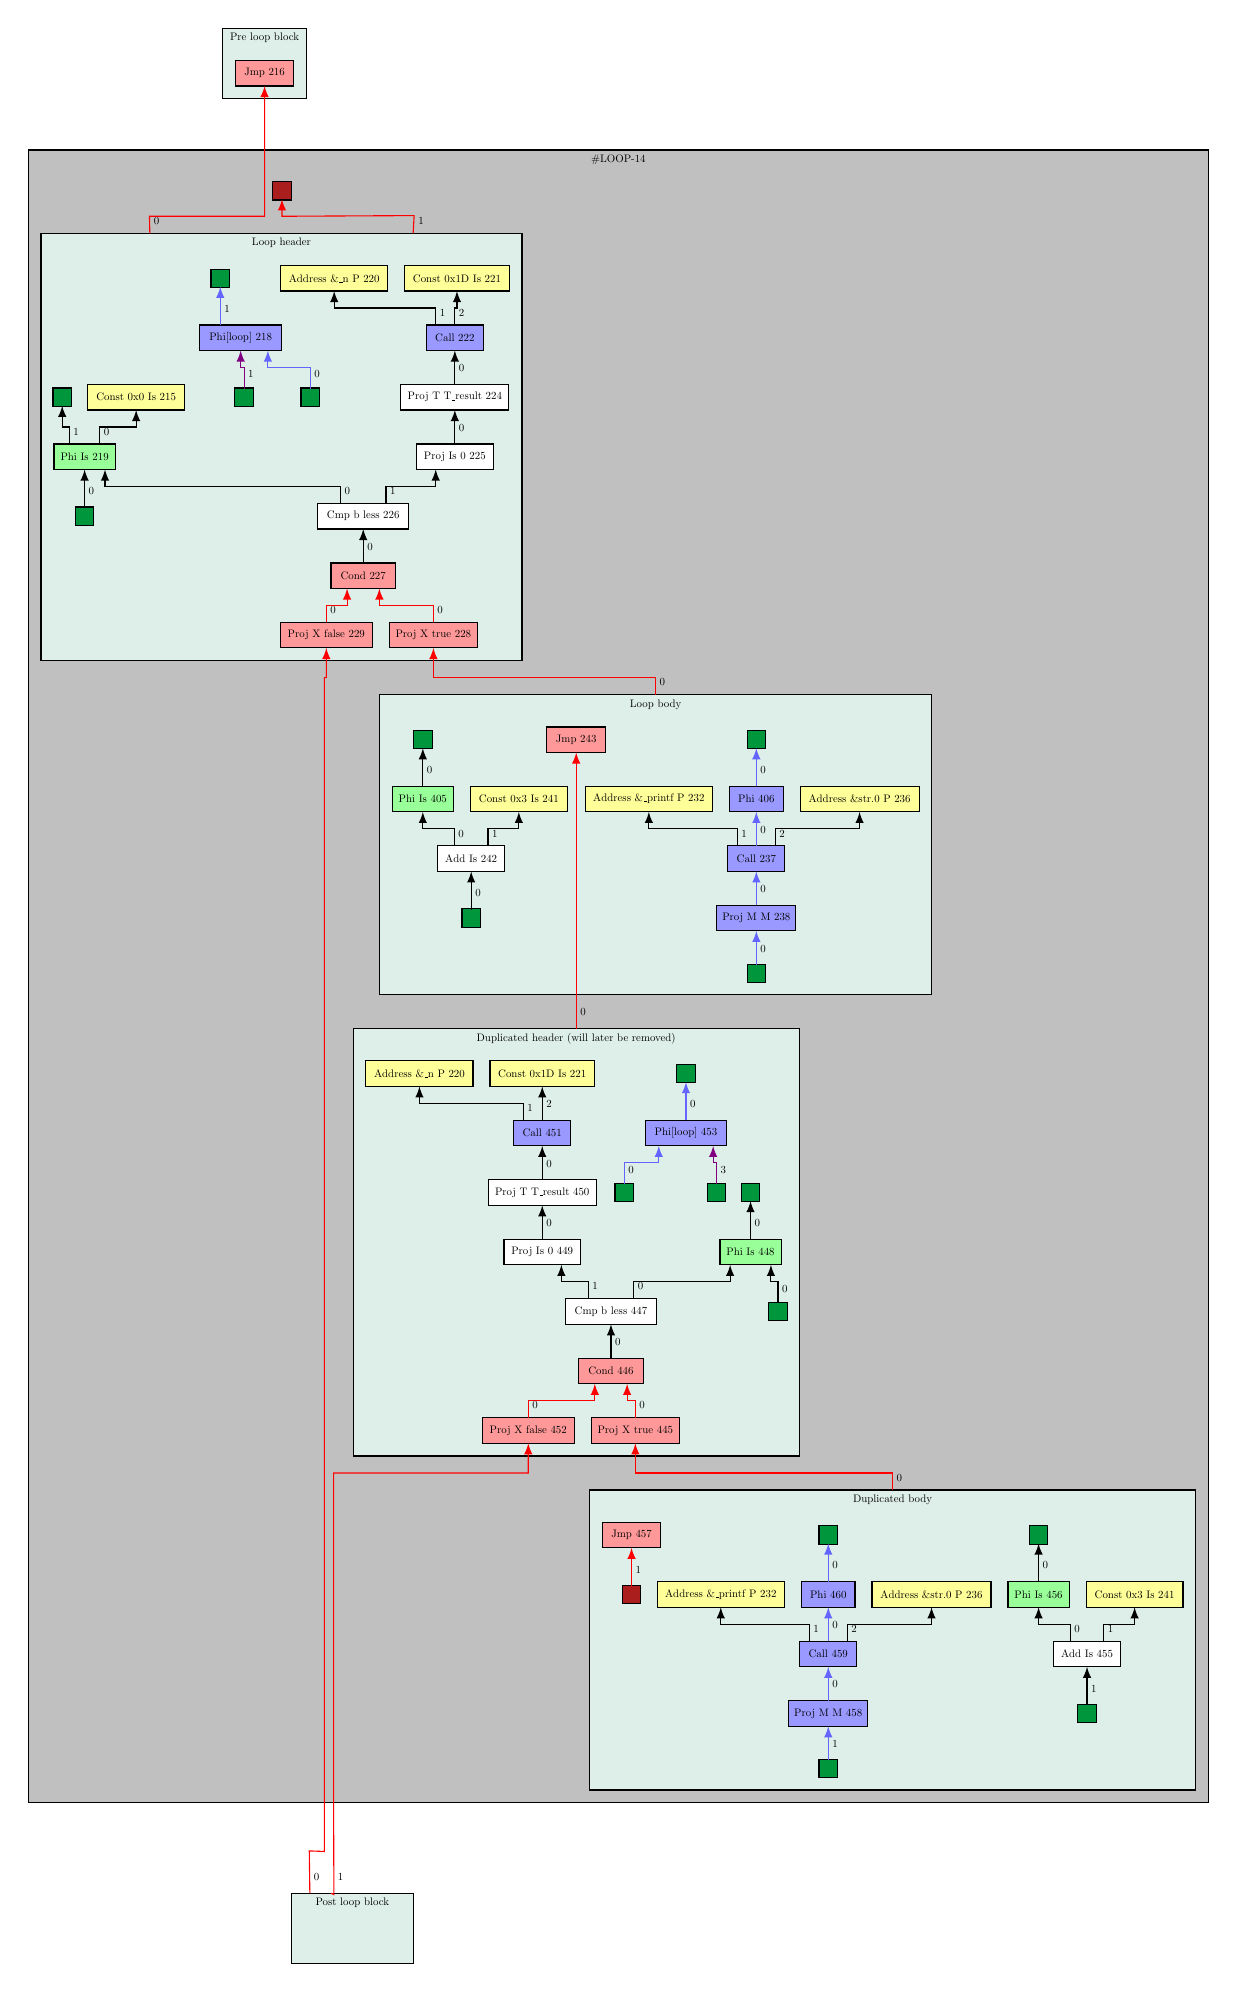
\begin{tikzpicture}
	\node[fill=color33, draw, minimum width=1.0683453237410072cm, minimum height=0.8956834532374102cm] (n101) at (11.222505742415636cm ,22.552094823164907cm) {};
	\node[fill=color34, draw, minimum width=14.989502857940924cm, minimum height=20.989208633093526cm] (n107) at (15.71598787432375cm ,10.958633093525181cm) {};
	% 1 node layouts
	\node[scale=0.3924133420536298, transform shape] at (11.222505742415636cm ,22.87667890589872cm) {Pre loop block};
	\node[fill=color33, draw, minimum width=7.699640287769787cm, minimum height=3.809352517985612cm] (n102) at (19.199048655812195cm ,2.5305755395683454cm) {};
	% 1 node layouts
	\node[scale=0.3924133420536298, transform shape] at (19.199048655812195cm ,4.311994154676259cm) {Duplicated body};
	\node[fill=color33, draw, minimum width=6.108812949640288cm, minimum height=5.428057553956835cm] (n103) at (11.437513423770554cm ,17.681654676258994cm) {};
	% 1 node layouts
	\node[scale=0.3924133420536298, transform shape] at (11.437513423770554cm ,20.27242580935252cm) {Loop header};
	\node[fill=color33, draw, minimum width=7.014388489208634cm, minimum height=3.809352517985612cm] (n104) at (16.189541668100926cm ,12.631294964028777cm) {};
	% 1 node layouts
	\node[scale=0.3924133420536298, transform shape] at (16.189541668100926cm ,14.41271357913669cm) {Loop body};
	\node[fill=color33, draw, minimum width=5.664977109221715cm, minimum height=5.428057553956835cm] (n105) at (15.18054886234553cm ,7.580935251798562cm) {};
	% 1 node layouts
	\node[scale=0.3924133420536298, transform shape] at (15.18054886234553cm ,10.171706384892087cm) {Duplicated header (will later be removed)};
	\node[fill=color33, draw, minimum width=1.5539568345323742cm, minimum height=0.8956834532374102cm] (n106) at (12.337230215827338cm ,-1.1337679856115108cm) {};
	% 1 node layouts
	\node[scale=0.3924133420536298, transform shape] at (12.337230215827338cm ,-0.8091839028776979cm) {Post loop block};
	% 1 node layouts
	\node[scale=0.3924133420536298, transform shape] at (15.71598787432375cm ,21.32997976618705cm) {\#LOOP-14};
	\node[fill=color35, draw, minimum width=0.7446043165467626cm, minimum height=0.32374100719424465cm] (n108) at (11.222505742415636cm ,22.427994103740446cm) {};
	% 1 node layouts
	\node[scale=0.3924133420536298, transform shape] at (11.222505742415636cm ,22.427994103740446cm) {Jmp  216};
	\node[fill=color36, draw, minimum width=1.0359712230215827cm, minimum height=0.32374100719424465cm] (n109) at (16.57429068706757cm ,8.967625899280575cm) {};
	% 1 node layouts
	\node[scale=0.3924133420536298, transform shape] at (16.57429068706757cm ,8.967625899280575cm) {Phi[loop]  453};
	\node[fill=color35, draw, minimum width=1.1654676258992807cm, minimum height=0.32374100719424465cm] (n110) at (14.571858541874635cm ,5.190647482014389cm) {};
	% 1 node layouts
	\node[scale=0.3924133420536298, transform shape] at (14.571858541874635cm ,5.190647482014389cm) {Proj X false 452};
	\node[fill=color35, draw, minimum width=1.1223021582733814cm, minimum height=0.32374100719424465cm] (n111) at (15.931570772090462cm ,5.190647482014389cm) {};
	% 1 node layouts
	\node[scale=0.3924133420536298, transform shape] at (15.931570772090462cm ,5.190647482014389cm) {Proj X true 445};
	\node[fill=color35, draw, minimum width=0.8201438848920863cm, minimum height=0.32374100719424465cm] (n112) at (15.62195255757117cm ,5.946043165467626cm) {};
	% 1 node layouts
	\node[scale=0.3924133420536298, transform shape] at (15.62195255757117cm ,5.946043165467626cm) {Cond  446};
	\node[fill=color37, draw, minimum width=1.154676258992806cm, minimum height=0.32374100719424465cm] (n113) at (15.62195255757117cm ,6.701438848920864cm) {};
	% 1 node layouts
	\node[scale=0.3924133420536298, transform shape] at (15.62195255757117cm ,6.701438848920864cm) {Cmp b less 447};
	\node[fill=color38, draw, minimum width=0.7769784172661871cm, minimum height=0.32374100719424465cm] (n114) at (17.394434571959657cm ,7.456834532374101cm) {};
	% 1 node layouts
	\node[scale=0.3924133420536298, transform shape] at (17.394434571959657cm ,7.456834532374101cm) {Phi Is 448};
	\node[fill=color37, draw, minimum width=0.9712230215827339cm, minimum height=0.32374100719424465cm] (n115) at (14.749139444425321cm ,7.456834532374101cm) {};
	% 1 node layouts
	\node[scale=0.3924133420536298, transform shape] at (14.749139444425321cm ,7.456834532374101cm) {Proj Is 0 449};
	\node[fill=color37, draw, minimum width=1.3705035971223023cm, minimum height=0.32374100719424465cm] (n116) at (14.749139444425321cm ,8.212230215827338cm) {};
	% 1 node layouts
	\node[scale=0.3924133420536298, transform shape] at (14.749139444425321cm ,8.212230215827338cm) {Proj T T\_result 450};
	\node[fill=color36, draw, minimum width=0.723021582733813cm, minimum height=0.32374100719424465cm] (n117) at (14.749139444425321cm ,8.967625899280575cm) {};
	% 1 node layouts
	\node[scale=0.3924133420536298, transform shape] at (14.749139444425321cm ,8.967625899280575cm) {Call  451};
	\node[fill=color39, draw, minimum width=1.3597122302158273cm, minimum height=0.32374100719424465cm] (n118) at (13.189786926439709cm ,9.723021582733814cm) {};
	% 1 node layouts
	\node[scale=0.3924133420536298, transform shape] at (13.189786926439709cm ,9.723021582733814cm) {Address \&\_n P 220};
	\node[fill=color39, draw, minimum width=1.3273381294964028cm, minimum height=0.32374100719424465cm] (n119) at (14.749139444425321cm ,9.723021582733814cm) {};
	% 1 node layouts
	\node[scale=0.3924133420536298, transform shape] at (14.749139444425321cm ,9.723021582733814cm) {Const 0x1D Is 221};
	\node[fill=color40, draw, minimum width=0.21582733812949642cm, minimum height=0.21582733812949642cm] (n120) at (15.79050635090014cm ,8.212230215827338cm) {};
	\node[fill=color40, draw, minimum width=0.21582733812949642cm, minimum height=0.21582733812949642cm] (n121) at (17.743253244294518cm ,6.701438848920864cm) {};
	\node[fill=color40, draw, minimum width=0.21582733812949642cm, minimum height=0.21582733812949642cm] (n122) at (16.57429068706757cm ,9.723021582733814cm) {};
	\node[fill=color40, draw, minimum width=0.21582733812949642cm, minimum height=0.21582733812949642cm] (n123) at (17.394434571959657cm ,8.212230215827338cm) {};
	\node[fill=color40, draw, minimum width=0.21582733812949642cm, minimum height=0.21582733812949642cm] (n124) at (16.962779895700667cm ,8.212230215827338cm) {};
	\node[fill=color36, draw, minimum width=1.0035971223021583cm, minimum height=0.32374100719424465cm] (n125) at (18.381602612646724cm ,1.5971223021582734cm) {};
	% 1 node layouts
	\node[scale=0.3924133420536298, transform shape] at (18.381602612646724cm ,1.5971223021582734cm) {Proj M M 458};
	\node[fill=color36, draw, minimum width=0.723021582733813cm, minimum height=0.32374100719424465cm] (n126) at (18.381602612646724cm ,2.352517985611511cm) {};
	% 1 node layouts
	\node[scale=0.3924133420536298, transform shape] at (18.381602612646724cm ,2.352517985611511cm) {Call  459};
	\node[fill=color39, draw, minimum width=1.6187050359712232cm, minimum height=0.32374100719424465cm] (n127) at (17.01649469897766cm ,3.1079136690647484cm) {};
	% 1 node layouts
	\node[scale=0.3924133420536298, transform shape] at (17.01649469897766cm ,3.1079136690647484cm) {Address \&\_printf P 232};
	\node[fill=color39, draw, minimum width=1.510791366906475cm, minimum height=0.32374100719424465cm] (n128) at (19.692753691783416cm ,3.1079136690647484cm) {};
	% 1 node layouts
	\node[scale=0.3924133420536298, transform shape] at (19.692753691783416cm ,3.1079136690647484cm) {Address \&str.0 P 236};
	\node[fill=color36, draw, minimum width=0.6798561151079137cm, minimum height=0.32374100719424465cm] (n129) at (18.381602612646724cm ,3.1079136690647484cm) {};
	% 1 node layouts
	\node[scale=0.3924133420536298, transform shape] at (18.381602612646724cm ,3.1079136690647484cm) {Phi  460};
	\node[fill=color35, draw, minimum width=0.7446043165467626cm, minimum height=0.32374100719424465cm] (n130) at (15.883401173797804cm ,3.863309352517986cm) {};
	% 1 node layouts
	\node[scale=0.3924133420536298, transform shape] at (15.883401173797804cm ,3.863309352517986cm) {Jmp  457};
	\node[fill=color37, draw, minimum width=0.8525179856115108cm, minimum height=0.32374100719424465cm] (n131) at (21.66795924162925cm ,2.352517985611511cm) {};
	% 1 node layouts
	\node[scale=0.3924133420536298, transform shape] at (21.66795924162925cm ,2.352517985611511cm) {Add Is 455};
	\node[fill=color39, draw, minimum width=1.2302158273381296cm, minimum height=0.32374100719424465cm] (n132) at (22.2718903824309cm ,3.1079136690647484cm) {};
	% 1 node layouts
	\node[scale=0.3924133420536298, transform shape] at (22.2718903824309cm ,3.1079136690647484cm) {Const 0x3 Is 241};
	\node[fill=color38, draw, minimum width=0.7769784172661871cm, minimum height=0.32374100719424465cm] (n133) at (21.052465921999243cm ,3.1079136690647484cm) {};
	% 1 node layouts
	\node[scale=0.3924133420536298, transform shape] at (21.052465921999243cm ,3.1079136690647484cm) {Phi Is 456};
	\node[fill=color40, draw, minimum width=0.21582733812949642cm, minimum height=0.21582733812949642cm] (n134) at (18.381602612646724cm ,3.863309352517986cm) {};
	\node[fill=color40, draw, minimum width=0.21582733812949642cm, minimum height=0.21582733812949642cm] (n135) at (21.052465921999243cm ,3.863309352517986cm) {};
	\node[fill=color40, draw, minimum width=0.21582733812949642cm, minimum height=0.21582733812949642cm] (n136) at (18.381602612646724cm ,0.8956834532374102cm) {};
	\node[fill=color40, draw, minimum width=0.21582733812949642cm, minimum height=0.21582733812949642cm] (n137) at (21.66795924162925cm ,1.5971223021582734cm) {};
	\node[fill=color36, draw, minimum width=1.0359712230215827cm, minimum height=0.32374100719424465cm] (n138) at (10.919078171971991cm ,19.06834532374101cm) {};
	% 1 node layouts
	\node[scale=0.3924133420536298, transform shape] at (10.919078171971991cm ,19.06834532374101cm) {Phi[loop]  218};
	\node[fill=color35, draw, minimum width=1.1654676258992807cm, minimum height=0.32374100719424465cm] (n139) at (12.006851703147051cm ,15.29136690647482cm) {};
	% 1 node layouts
	\node[scale=0.3924133420536298, transform shape] at (12.006851703147051cm ,15.29136690647482cm) {Proj X false 229};
	\node[fill=color35, draw, minimum width=1.1223021582733814cm, minimum height=0.32374100719424465cm] (n140) at (13.366563933362878cm ,15.29136690647482cm) {};
	% 1 node layouts
	\node[scale=0.3924133420536298, transform shape] at (13.366563933362878cm ,15.29136690647482cm) {Proj X true 228};
	\node[fill=color35, draw, minimum width=0.8201438848920863cm, minimum height=0.32374100719424465cm] (n141) at (12.475732848230985cm ,16.046762589928058cm) {};
	% 1 node layouts
	\node[scale=0.3924133420536298, transform shape] at (12.475732848230985cm ,16.046762589928058cm) {Cond  227};
	\node[fill=color37, draw, minimum width=1.154676258992806cm, minimum height=0.32374100719424465cm] (n142) at (12.475732848230985cm ,16.802158273381295cm) {};
	% 1 node layouts
	\node[scale=0.3924133420536298, transform shape] at (12.475732848230985cm ,16.802158273381295cm) {Cmp b less 226};
	\node[fill=color37, draw, minimum width=0.9712230215827339cm, minimum height=0.32374100719424465cm] (n143) at (13.63915835782331cm ,17.557553956834532cm) {};
	% 1 node layouts
	\node[scale=0.3924133420536298, transform shape] at (13.63915835782331cm ,17.557553956834532cm) {Proj Is 0 225};
	\node[fill=color37, draw, minimum width=1.3705035971223023cm, minimum height=0.32374100719424465cm] (n144) at (13.63915835782331cm ,18.31294964028777cm) {};
	% 1 node layouts
	\node[scale=0.3924133420536298, transform shape] at (13.63915835782331cm ,18.31294964028777cm) {Proj T T\_result 224};
	\node[fill=color36, draw, minimum width=0.723021582733813cm, minimum height=0.32374100719424465cm] (n145) at (13.63915835782331cm ,19.06834532374101cm) {};
	% 1 node layouts
	\node[scale=0.3924133420536298, transform shape] at (13.63915835782331cm ,19.06834532374101cm) {Call  222};
	\node[fill=color39, draw, minimum width=1.3597122302158273cm, minimum height=0.32374100719424465cm] (n146) at (12.10702781225976cm ,19.823741007194247cm) {};
	% 1 node layouts
	\node[scale=0.3924133420536298, transform shape] at (12.10702781225976cm ,19.823741007194247cm) {Address \&\_n P 220};
	\node[fill=color39, draw, minimum width=1.3273381294964028cm, minimum height=0.32374100719424465cm] (n147) at (13.666380330245373cm ,19.823741007194247cm) {};
	% 1 node layouts
	\node[scale=0.3924133420536298, transform shape] at (13.666380330245373cm ,19.823741007194247cm) {Const 0x1D Is 221};
	\node[fill=color38, draw, minimum width=0.7769784172661871cm, minimum height=0.32374100719424465cm] (n148) at (8.937157458542735cm ,17.557553956834532cm) {};
	% 1 node layouts
	\node[scale=0.3924133420536298, transform shape] at (8.937157458542735cm ,17.557553956834532cm) {Phi Is 219};
	\node[fill=color39, draw, minimum width=1.2302158273381296cm, minimum height=0.32374100719424465cm] (n149) at (9.591740042475589cm ,18.31294964028777cm) {};
	% 1 node layouts
	\node[scale=0.3924133420536298, transform shape] at (9.591740042475589cm ,18.31294964028777cm) {Const 0x0 Is 215};
	\node[fill=color40, draw, minimum width=0.21582733812949642cm, minimum height=0.21582733812949642cm] (n150) at (10.660085366216595cm ,19.823741007194247cm) {};
	\node[fill=color40, draw, minimum width=0.21582733812949642cm, minimum height=0.21582733812949642cm] (n151) at (8.65289112161228cm ,18.31294964028777cm) {};
	\node[fill=color40, draw, minimum width=0.21582733812949642cm, minimum height=0.21582733812949642cm] (n152) at (11.802902362619474cm ,18.31294964028777cm) {};
	\node[fill=color40, draw, minimum width=0.21582733812949642cm, minimum height=0.21582733812949642cm] (n153) at (8.937157458542735cm ,16.802158273381295cm) {};
	\node[fill=color40, draw, minimum width=0.21582733812949642cm, minimum height=0.21582733812949642cm] (n154) at (10.96224363959789cm ,18.31294964028777cm) {};
	\node[fill=color36, draw, minimum width=1.0035971223021583cm, minimum height=0.32374100719424465cm] (n155) at (17.468318646518192cm ,11.697841726618705cm) {};
	% 1 node layouts
	\node[scale=0.3924133420536298, transform shape] at (17.468318646518192cm ,11.697841726618705cm) {Proj M M 238};
	\node[fill=color36, draw, minimum width=0.723021582733813cm, minimum height=0.32374100719424465cm] (n156) at (17.468318646518192cm ,12.453237410071942cm) {};
	% 1 node layouts
	\node[scale=0.3924133420536298, transform shape] at (17.468318646518192cm ,12.453237410071942cm) {Call  237};
	\node[fill=color39, draw, minimum width=1.6187050359712232cm, minimum height=0.32374100719424465cm] (n157) at (16.103210732849128cm ,13.208633093525181cm) {};
	% 1 node layouts
	\node[scale=0.3924133420536298, transform shape] at (16.103210732849128cm ,13.208633093525181cm) {Address \&\_printf P 232};
	\node[fill=color39, draw, minimum width=1.510791366906475cm, minimum height=0.32374100719424465cm] (n158) at (18.77946972565488cm ,13.208633093525181cm) {};
	% 1 node layouts
	\node[scale=0.3924133420536298, transform shape] at (18.77946972565488cm ,13.208633093525181cm) {Address \&str.0 P 236};
	\node[fill=color36, draw, minimum width=0.6798561151079137cm, minimum height=0.32374100719424465cm] (n159) at (17.468318646518192cm ,13.208633093525181cm) {};
	% 1 node layouts
	\node[scale=0.3924133420536298, transform shape] at (17.468318646518192cm ,13.208633093525181cm) {Phi  406};
	\node[fill=color35, draw, minimum width=0.7446043165467626cm, minimum height=0.32374100719424465cm] (n160) at (15.18054886234553cm ,13.964028776978418cm) {};
	% 1 node layouts
	\node[scale=0.3924133420536298, transform shape] at (15.18054886234553cm ,13.964028776978418cm) {Jmp  243};
	\node[fill=color37, draw, minimum width=0.8525179856115108cm, minimum height=0.32374100719424465cm] (n161) at (13.84691576882035cm ,12.453237410071942cm) {};
	% 1 node layouts
	\node[scale=0.3924133420536298, transform shape] at (13.84691576882035cm ,12.453237410071942cm) {Add Is 242};
	\node[fill=color39, draw, minimum width=1.2302158273381296cm, minimum height=0.32374100719424465cm] (n162) at (14.452131596158479cm ,13.208633093525181cm) {};
	% 1 node layouts
	\node[scale=0.3924133420536298, transform shape] at (14.452131596158479cm ,13.208633093525181cm) {Const 0x3 Is 241};
	\node[fill=color38, draw, minimum width=0.7769784172661871cm, minimum height=0.32374100719424465cm] (n163) at (13.232707135726825cm ,13.208633093525181cm) {};
	% 1 node layouts
	\node[scale=0.3924133420536298, transform shape] at (13.232707135726825cm ,13.208633093525181cm) {Phi Is 405};
	\node[fill=color40, draw, minimum width=0.21582733812949642cm, minimum height=0.21582733812949642cm] (n164) at (17.468318646518192cm ,13.964028776978418cm) {};
	\node[fill=color40, draw, minimum width=0.21582733812949642cm, minimum height=0.21582733812949642cm] (n165) at (13.232707135726825cm ,13.964028776978418cm) {};
	\node[fill=color40, draw, minimum width=0.21582733812949642cm, minimum height=0.21582733812949642cm] (n166) at (17.468318646518192cm ,10.996402877697843cm) {};
	\node[fill=color40, draw, minimum width=0.21582733812949642cm, minimum height=0.21582733812949642cm] (n167) at (13.84691576882035cm ,11.697841726618705cm) {};
	\node[fill=color41, draw, minimum width=0.21582733812949642cm, minimum height=0.21582733812949642cm] (n168) at (11.44372876399837cm ,20.93525179856115cm) {};
	\node[fill=color41, draw, minimum width=0.21582733812949642cm, minimum height=0.21582733812949642cm] (n169) at (15.883401173797804cm ,3.1079136690647484cm) {};
	\draw[color=color42, -latex] (19.199048655812195cm ,4.4352517985611515cm) -- (19.19904865581219cm ,4.651079136690647cm) -- (15.931570772090462cm ,4.651079136690647cm) -- (15.931570772090462cm ,5.028776978417266cm);
	\node[] at (19.285379591063993cm ,4.592401079136691cm) {
		\scalebox{0.3924133420536298}{0}
	};
	\draw[color=color42, -latex] (9.7655494324636cm ,20.39568345323741cm) -- (9.760920011000769cm ,20.611510791366907cm) -- (11.222505742415636cm ,20.611510791366907cm) -- (11.222505742415636cm ,22.266123600143324cm);
	\node[] at (9.850608180996998cm ,20.552832733812952cm) {
		\scalebox{0.3924133420536298}{0}
	};
	\draw[color=color42, -latex] (16.189541668100926cm ,14.535971223021583cm) -- (16.189541668100926cm ,14.75179856115108cm) -- (13.366563933362878cm ,14.75179856115108cm) -- (13.366563933362878cm ,15.129496402877699cm);
	\node[] at (16.275872603352724cm ,14.693120503597124cm) {
		\scalebox{0.3924133420536298}{0}
	};
	\draw[color=color42, -latex] (15.18054886234553cm ,10.29496402877698cm) -- (15.18054886234553cm ,13.802158273381295cm);
	\node[] at (15.266879797597328cm ,10.502065535071942cm) {
		\scalebox{0.3924133420536298}{0}
	};
	\draw[color=color42, -latex] (11.797661870503598cm ,-0.6858714590827368cm) -- (11.790546954690896cm ,-0.14814226901732497cm) -- (11.981892086330935cm ,-0.15513669064747931cm) -- (11.981545385701008cm ,0.24820143884892087cm) -- (11.981545385701008cm ,14.75179856115108cm) -- (12.006851703147051cm ,14.75179856115108cm) -- (12.006851703147051cm ,15.129496402877699cm);
	\node[] at (11.88254783262315cm ,-0.47882475269784175cm) {
		\scalebox{0.3924133420536298}{0}
	};
	\draw[color=color42, -latex] (12.067446043165468cm ,-0.6858714590827368cm) -- (12.103153327338127cm ,-0.7027877697841727cm) -- (12.100250421672232cm ,0.14028776978417268cm) -- (12.100250421672232cm ,4.651079136690647cm) -- (14.571858541874635cm ,4.651079136690647cm) -- (14.571858541874635cm ,5.028776978417266cm);
	\node[] at (12.189049987902306cm ,-0.47882475269784175cm) {
		\scalebox{0.3924133420536298}{1}
	};
	\draw[color=color43, -latex] (16.57429068706757cm ,9.129496402877699cm) -- (16.57429068706757cm ,9.615107913669066cm);
	\node[] at (16.660621622319372cm ,9.336597909172662cm) {
		\scalebox{0.3924133420536298}{0}
	};
	\draw[color=color42, -latex] (14.571858541874635cm ,5.352517985611511cm) -- (14.571858541874635cm ,5.568345323741007cm) -- (15.416916586348147cm ,5.568345323741007cm) -- (15.416916586348147cm ,5.784172661870504cm);
	\node[] at (14.658189477126433cm ,5.5096672661870505cm) {
		\scalebox{0.3924133420536298}{0}
	};
	\draw[color=color42, -latex] (15.931570772090462cm ,5.352517985611511cm) -- (15.931570772090462cm ,5.568345323741007cm) -- (15.82698852879419cm ,5.568345323741007cm) -- (15.82698852879419cm ,5.784172661870504cm);
	\node[] at (16.01790170734226cm ,5.5096672661870505cm) {
		\scalebox{0.3924133420536298}{0}
	};
	\draw[color=color44, -latex] (15.62195255757117cm ,6.107913669064748cm) -- (15.62195255757117cm ,6.539568345323741cm);
	\node[] at (15.708283492822968cm ,6.315015175359712cm) {
		\scalebox{0.3924133420536298}{0}
	};
	\draw[color=color44, -latex] (15.91062162231937cm ,6.863309352517986cm) -- (15.91062162231937cm ,7.079136690647482cm) -- (17.135441766204263cm ,7.079136690647482cm) -- (17.135441766204263cm ,7.294964028776978cm);
	\node[] at (15.99695255757117cm ,7.020458633093526cm) {
		\scalebox{0.3924133420536298}{0}
	};
	\draw[color=color44, -latex] (15.333283492822968cm ,6.863309352517986cm) -- (15.333283492822968cm ,7.079136690647482cm) -- (14.991945199821004cm ,7.079136690647482cm) -- (14.991945199821004cm ,7.294964028776978cm);
	\node[] at (15.419614428074766cm ,7.020458633093526cm) {
		\scalebox{0.3924133420536298}{1}
	};
	\draw[color=color44, -latex] (17.394434571959657cm ,7.618705035971224cm) -- (17.394434571959657cm ,8.10431654676259cm);
	\node[] at (17.48076550721146cm ,7.8258065422661875cm) {
		\scalebox{0.3924133420536298}{0}
	};
	\draw[color=color44, -latex] (14.749139444425321cm ,7.618705035971224cm) -- (14.749139444425321cm ,8.050359712230216cm);
	\node[] at (14.835470379677119cm ,7.8258065422661875cm) {
		\scalebox{0.3924133420536298}{0}
	};
	\draw[color=color44, -latex] (14.749139444425321cm ,8.374100719424462cm) -- (14.749139444425321cm ,8.805755395683454cm);
	\node[] at (14.835470379677119cm ,8.581202225719425cm) {
		\scalebox{0.3924133420536298}{0}
	};
	\draw[color=color44, -latex] (14.508132250180717cm ,9.129496402877699cm) -- (14.508132250180717cm ,9.345323741007194cm) -- (13.189786926439709cm ,9.345323741007194cm) -- (13.189786926439709cm ,9.56115107913669cm);
	\node[] at (14.594463185432515cm ,9.286645683453237cm) {
		\scalebox{0.3924133420536298}{1}
	};
	\draw[color=color44, -latex] (14.749139444425321cm ,9.129496402877699cm) -- (14.749139444425321cm ,9.56115107913669cm);
	\node[] at (14.835470379677119cm ,9.336597909172662cm) {
		\scalebox{0.3924133420536298}{2}
	};
	\draw[color=color43, -latex] (15.79050635090014cm ,8.320143884892087cm) -- (15.79050635090014cm ,8.589928057553957cm) -- (16.22896694606038cm ,8.589928057553957cm) -- (16.22896694606038cm ,8.805755395683454cm);
	\node[] at (15.87683728615194cm ,8.504271582733814cm) {
		\scalebox{0.3924133420536298}{0}
	};
	\draw[color=color44, -latex] (17.743253244294518cm ,6.809352517985612cm) -- (17.743253244294518cm ,7.079136690647482cm) -- (17.653427377715055cm ,7.079136690647482cm) -- (17.653427377715055cm ,7.294964028776978cm);
	\node[] at (17.829584179546316cm ,6.993480215827338cm) {
		\scalebox{0.3924133420536298}{0}
	};
	\draw[color=color45, -latex] (16.962779895700667cm ,8.320143884892087cm) -- (16.962779895700667cm ,8.589928057553957cm) -- (16.919614428074766cm ,8.589928057553957cm) -- (16.919614428074766cm ,8.805755395683454cm);
	\node[] at (17.049110830952465cm ,8.504271582733814cm) {
		\scalebox{0.3924133420536298}{3}
	};
	\draw[color=color43, -latex] (18.381602612646724cm ,1.7589928057553958cm) -- (18.381602612646724cm ,2.1906474820143886cm);
	\node[] at (18.467933547898525cm ,1.9660943120503598cm) {
		\scalebox{0.3924133420536298}{0}
	};
	\draw[color=color43, -latex] (18.381602612646724cm ,2.514388489208633cm) -- (18.381602612646724cm ,2.9460431654676262cm);
	\node[] at (18.467933547898525cm ,2.7214899955035974cm) {
		\scalebox{0.3924133420536298}{0}
	};
	\draw[color=color44, -latex] (18.14059541840212cm ,2.514388489208633cm) -- (18.14059541840212cm ,2.73021582733813cm) -- (17.01649469897766cm ,2.73021582733813cm) -- (17.01649469897766cm ,2.9460431654676262cm);
	\node[] at (18.22692635365392cm ,2.6715377697841727cm) {
		\scalebox{0.3924133420536298}{1}
	};
	\draw[color=color44, -latex] (18.62260980689133cm ,2.514388489208633cm) -- (18.62260980689133cm ,2.73021582733813cm) -- (19.692753691783416cm ,2.73021582733813cm) -- (19.692753691783416cm ,2.9460431654676262cm);
	\node[] at (18.708940742143128cm ,2.6715377697841727cm) {
		\scalebox{0.3924133420536298}{2}
	};
	\draw[color=color43, -latex] (18.381602612646724cm ,3.2697841726618706cm) -- (18.381602612646724cm ,3.7553956834532376cm);
	\node[] at (18.467933547898525cm ,3.4768856789568345cm) {
		\scalebox{0.3924133420536298}{0}
	};
	\draw[color=color44, -latex] (21.454829745226377cm ,2.514388489208633cm) -- (21.454829745226377cm ,2.73021582733813cm) -- (21.052465921999243cm ,2.73021582733813cm) -- (21.052465921999243cm ,2.9460431654676262cm);
	\node[] at (21.541160680478175cm ,2.6715377697841727cm) {
		\scalebox{0.3924133420536298}{0}
	};
	\draw[color=color44, -latex] (21.88108873803213cm ,2.514388489208633cm) -- (21.88108873803213cm ,2.73021582733813cm) -- (22.2718903824309cm ,2.73021582733813cm) -- (22.2718903824309cm ,2.9460431654676262cm);
	\node[] at (21.967419673283928cm ,2.6715377697841727cm) {
		\scalebox{0.3924133420536298}{1}
	};
	\draw[color=color44, -latex] (21.052465921999243cm ,3.2697841726618706cm) -- (21.052465921999243cm ,3.7553956834532376cm);
	\node[] at (21.13879685725104cm ,3.4768856789568345cm) {
		\scalebox{0.3924133420536298}{0}
	};
	\draw[color=color43, -latex] (18.381602612646724cm ,1.0035971223021583cm) -- (18.381602612646724cm ,1.4352517985611513cm);
	\node[] at (18.467933547898525cm ,1.2106986285971224cm) {
		\scalebox{0.3924133420536298}{1}
	};
	\draw[color=color44, -latex] (21.66795924162925cm ,1.7050359712230216cm) -- (21.66795924162925cm ,2.1906474820143886cm);
	\node[] at (21.754290176881053cm ,1.9121374775179858cm) {
		\scalebox{0.3924133420536298}{1}
	};
	\draw[color=color43, -latex] (10.660085366216595cm ,19.23021582733813cm) -- (10.660085366216595cm ,19.715827338129497cm);
	\node[] at (10.746416301468393cm ,19.437317333633093cm) {
		\scalebox{0.3924133420536298}{1}
	};
	\draw[color=color42, -latex] (12.006851703147051cm ,15.453237410071944cm) -- (12.006851703147051cm ,15.66906474820144cm) -- (12.270696877007962cm ,15.66906474820144cm) -- (12.270696877007962cm ,15.884892086330936cm);
	\node[] at (12.093182638398849cm ,15.610386690647482cm) {
		\scalebox{0.3924133420536298}{0}
	};
	\draw[color=color42, -latex] (13.366563933362878cm ,15.453237410071944cm) -- (13.366563933362878cm ,15.66906474820144cm) -- (12.680768819454006cm ,15.66906474820144cm) -- (12.680768819454006cm ,15.884892086330936cm);
	\node[] at (13.452894868614676cm ,15.610386690647482cm) {
		\scalebox{0.3924133420536298}{0}
	};
	\draw[color=color44, -latex] (12.475732848230985cm ,16.20863309352518cm) -- (12.475732848230985cm ,16.640287769784173cm);
	\node[] at (12.562063783482783cm ,16.415734599820144cm) {
		\scalebox{0.3924133420536298}{0}
	};
	\draw[color=color44, -latex] (12.187063783482783cm ,16.964028776978417cm) -- (12.187063783482783cm ,17.179856115107913cm) -- (9.196150264298131cm ,17.179856115107913cm) -- (9.196150264298131cm ,17.39568345323741cm);
	\node[] at (12.27339471873458cm ,17.12117805755396cm) {
		\scalebox{0.3924133420536298}{0}
	};
	\draw[color=color44, -latex] (12.764401912979185cm ,16.964028776978417cm) -- (12.764401912979185cm ,17.179856115107913cm) -- (13.396352602427626cm ,17.179856115107913cm) -- (13.396352602427626cm ,17.39568345323741cm);
	\node[] at (12.850732848230985cm ,17.12117805755396cm) {
		\scalebox{0.3924133420536298}{1}
	};
	\draw[color=color44, -latex] (13.63915835782331cm ,17.719424460431657cm) -- (13.63915835782331cm ,18.151079136690647cm);
	\node[] at (13.725489293075109cm ,17.92652596672662cm) {
		\scalebox{0.3924133420536298}{0}
	};
	\draw[color=color44, -latex] (13.63915835782331cm ,18.474820143884894cm) -- (13.63915835782331cm ,18.906474820143885cm);
	\node[] at (13.725489293075109cm ,18.681921650179856cm) {
		\scalebox{0.3924133420536298}{0}
	};
	\draw[color=color44, -latex] (13.398151163578707cm ,19.23021582733813cm) -- (13.398151163578707cm ,19.44604316546763cm) -- (12.10702781225976cm ,19.44604316546763cm) -- (12.10702781225976cm ,19.66187050359712cm);
	\node[] at (13.484482098830506cm ,19.38736510791367cm) {
		\scalebox{0.3924133420536298}{1}
	};
	\draw[color=color44, -latex] (13.63915835782331cm ,19.23021582733813cm) -- (13.63915835782331cm ,19.44604316546763cm) -- (13.666380330245373cm ,19.44604316546763cm) -- (13.666380330245373cm ,19.66187050359712cm);
	\node[] at (13.725489293075109cm ,19.38736510791367cm) {
		\scalebox{0.3924133420536298}{2}
	};
	\draw[color=color44, -latex] (9.131402062859282cm ,17.719424460431657cm) -- (9.131402062859282cm ,17.93525179856115cm) -- (9.591740042475589cm ,17.93525179856115cm) -- (9.591740042475589cm ,18.151079136690647cm);
	\node[] at (9.21773299811108cm ,17.876573741007196cm) {
		\scalebox{0.3924133420536298}{0}
	};
	\draw[color=color44, -latex] (8.742912854226187cm ,17.719424460431657cm) -- (8.742912854226187cm ,17.93525179856115cm) -- (8.65289112161228cm ,17.93525179856115cm) -- (8.65289112161228cm ,18.205035971223023cm);
	\node[] at (8.829243789477987cm ,17.876573741007196cm) {
		\scalebox{0.3924133420536298}{1}
	};
	\draw[color=color43, -latex] (11.802902362619474cm ,18.42086330935252cm) -- (11.802902362619474cm ,18.690647482014388cm) -- (11.264401912979185cm ,18.690647482014388cm) -- (11.264401912979185cm ,18.906474820143885cm);
	\node[] at (11.889233297871273cm ,18.604991007194247cm) {
		\scalebox{0.3924133420536298}{0}
	};
	\draw[color=color44, -latex] (8.937157458542735cm ,16.910071942446045cm) -- (8.937157458542735cm ,17.39568345323741cm);
	\node[] at (9.023488393794533cm ,17.117173448741006cm) {
		\scalebox{0.3924133420536298}{0}
	};
	\draw[color=color45, -latex] (10.96224363959789cm ,18.42086330935252cm) -- (10.96224363959789cm ,18.690647482014388cm) -- (10.919078171971991cm ,18.690647482014388cm) -- (10.919078171971991cm ,18.906474820143885cm);
	\node[] at (11.048574574849688cm ,18.604991007194247cm) {
		\scalebox{0.3924133420536298}{1}
	};
	\draw[color=color43, -latex] (17.468318646518192cm ,11.859712230215829cm) -- (17.468318646518192cm ,12.29136690647482cm);
	\node[] at (17.55464958176999cm ,12.066813736510792cm) {
		\scalebox{0.3924133420536298}{0}
	};
	\draw[color=color43, -latex] (17.468318646518192cm ,12.615107913669066cm) -- (17.468318646518192cm ,13.046762589928058cm);
	\node[] at (17.55464958176999cm ,12.822209419964029cm) {
		\scalebox{0.3924133420536298}{0}
	};
	\draw[color=color44, -latex] (17.22731145227359cm ,12.615107913669066cm) -- (17.22731145227359cm ,12.830935251798563cm) -- (16.103210732849128cm ,12.830935251798563cm) -- (16.103210732849128cm ,13.046762589928058cm);
	\node[] at (17.313642387525388cm ,12.772257194244604cm) {
		\scalebox{0.3924133420536298}{1}
	};
	\draw[color=color44, -latex] (17.709325840762794cm ,12.615107913669066cm) -- (17.709325840762794cm ,12.830935251798563cm) -- (18.77946972565488cm ,12.830935251798563cm) -- (18.77946972565488cm ,13.046762589928058cm);
	\node[] at (17.795656776014592cm ,12.772257194244604cm) {
		\scalebox{0.3924133420536298}{2}
	};
	\draw[color=color43, -latex] (17.468318646518192cm ,13.370503597122303cm) -- (17.468318646518192cm ,13.85611510791367cm);
	\node[] at (17.55464958176999cm ,13.577605103417266cm) {
		\scalebox{0.3924133420536298}{0}
	};
	\draw[color=color44, -latex] (13.633786272417472cm ,12.615107913669066cm) -- (13.633786272417472cm ,12.830935251798563cm) -- (13.232707135726825cm ,12.830935251798563cm) -- (13.232707135726825cm ,13.046762589928058cm);
	\node[] at (13.720117207669272cm ,12.772257194244604cm) {
		\scalebox{0.3924133420536298}{0}
	};
	\draw[color=color44, -latex] (14.060045265223229cm ,12.615107913669066cm) -- (14.060045265223229cm ,12.830935251798563cm) -- (14.452131596158479cm ,12.830935251798563cm) -- (14.452131596158479cm ,13.046762589928058cm);
	\node[] at (14.146376200475027cm ,12.772257194244604cm) {
		\scalebox{0.3924133420536298}{1}
	};
	\draw[color=color44, -latex] (13.232707135726825cm ,13.370503597122303cm) -- (13.232707135726825cm ,13.85611510791367cm);
	\node[] at (13.319038070978623cm ,13.577605103417266cm) {
		\scalebox{0.3924133420536298}{0}
	};
	\draw[color=color43, -latex] (17.468318646518192cm ,11.10431654676259cm) -- (17.468318646518192cm ,11.535971223021583cm);
	\node[] at (17.55464958176999cm ,11.311418053057555cm) {
		\scalebox{0.3924133420536298}{0}
	};
	\draw[color=color44, -latex] (13.84691576882035cm ,11.805755395683454cm) -- (13.84691576882035cm ,12.29136690647482cm);
	\node[] at (13.933246704072149cm ,12.012856901978418cm) {
		\scalebox{0.3924133420536298}{0}
	};
	\draw[color=color42, -latex] (13.109477415077507cm ,20.39568345323741cm) -- (13.122114180665038cm ,20.620143884892087cm) -- (11.44372876399837cm ,20.611510791366907cm) -- (11.44372876399837cm ,20.827338129496404cm);
	\node[] at (13.210406795310364cm ,20.55714928057554cm) {
		\scalebox{0.3924133420536298}{1}
	};
	\draw[color=color42, -latex] (15.883401173797804cm ,3.2158273381294964cm) -- (15.883401173797804cm ,3.7014388489208634cm);
	\node[] at (15.969732109049604cm ,3.4229288444244608cm) {
		\scalebox{0.3924133420536298}{1}
	};
\end{tikzpicture}

    \end{adjustbox}
    \caption{Firm graph of the loop shown in \cref{fig:impl:unroll:unroll-factor-2-before} unrolled with a factor of two}
    \label{fig:impl:unroll:unroll-factor-2-after}
\end{figure}